\section{Installation, update, use}

{\setbeamercolor{background canvas}{bg=LemonChiffon}
\begin{frame}
\frametitle{}
{\fontsize{50}{60}\selectfont Installation\\
 \& use} 

\end{frame}
}


\subsection{Installing}

\begin{frame}
\frametitle{Installing Python}

\begin{description}

\item<1->[Hard way:] download source and compile:\\
\url{https://www.python.org/downloads/}

\item<2->[Normal way:] use installer or package:

\begin{itemize}
\item Windows: \url{https://www.python.org/downloads/windows/}
\item Mac OS: \url{https://www.python.org/downloads/mac-osx/}
\item Linux: package manager:\\
python2.x and python2.x-dev packages
\end{itemize}

\item<3->[Easy way:] Python distributions such as:\\
\href{https://www.continuum.io/downloads}{Anaconda} \comment{free}\\
\href{https://www.enthought.com/products/canopy/}{Enthought Canopy} \comment{free and commercial}\\
\href{http://python-xy.github.io/}{Python(x,y)} \comment{free, Windows only}\\
+ others

\end{description}

\end{frame}

%--------------------------------------------------------------------------------------------------------------
\begin{frame}[fragile]
\frametitle{Installing modules}

Example: SciPy (\url{http://www.scipy.org/}):\\
mathematics, science, and engineering

\begin{description}
\item<2->[Easy way:] Windows, Linux, Mac:\\
use Scientific Python distribution
\item<3->[Intermediate:] Linux, Mac: install package\\
\begin{itemize}
\item Linux: package manager
\item Mac: \href{https://www.macports.org/}{MacPorts}, \href{http://brew.sh/}{Homebrew}
\end{itemize}
\item<4->[Harder:] build from source
\begin{lstlisting}[language=bash]
 $ python setup.py install
\end{lstlisting}
\item<5->[Better:] pip (\url{https://pypi.python.org/pypi/pip})
\item<6->[Avoid:] mixing installation methods

\end{description}

\end{frame}


%--------------------------------------------------------------------------------------------------------------
\begin{frame}[fragile]
\frametitle{Using \texttt{pip} to manage modules}

\texttt{pip} = recommended tool for installing Python packages

\begin{description}
\item<2->[Installation:]
\begin{itemize}
\item Included in recent Python version
\item Otherwise: download and run \pyfile{get-pip.py}\\
\url{https://pip.pypa.io/en/stable/installing/\#install-pip}
\begin{lstlisting}[language=bash]
$ python get-pip.py
\end{lstlisting}
\end{itemize}

\item<3->[Usage:]
\begin{itemize}
\item Install latest version + dependencies:
\begin{lstlisting}[language=bash]
$ pip install Package
\end{lstlisting}

\item Specify exact version:
\begin{lstlisting}[language=bash]
$ pip install Package==x.y.z
\end{lstlisting}
\item Specify minimum version:
\begin{lstlisting}[language=bash]
$ pip install 'Package>=x.y.z'
\end{lstlisting}
\end{itemize}

\end{description}

\end{frame}

%--------------------------------------------------------------------------------------------------------------
\begin{frame}[t, fragile]
\frametitle{More about \texttt{pip}}


\begin{itemize}
\item<1-> Uninstall packages:                   
\begin{lstlisting}[language=bash]
$ pip uninstall
\end{lstlisting}
\item<2->List installed packages:
\begin{lstlisting}[language=bash]
$ pip list
\end{lstlisting}

\begin{onlyenv}<2>
\tiny
\begin{lstlisting}[language=bash]
aptoncd (0.1.98-bzr117-1.2)
backports.ssl-match-hostname (3.4.0.2)
basemap (1.0.7)
...
xhtml2pdf (0.0.6)
zope.interface (3.6.1)
\end{lstlisting}
\end{onlyenv}


\item<3-> Output installed packages in requirements format:
\begin{lstlisting}[language=bash]
$ pip freeze
\end{lstlisting}

\begin{onlyenv}<3>
\tiny
\begin{lstlisting}[language=bash]
aptoncd===0.1.98-bzr117-1.2
backports.ssl-match-hostname==3.4.0.2
basemap==1.0.7

...
xhtml2pdf==0.0.6
zope.interface==3.6.1
\end{lstlisting}
\end{onlyenv}

\item<4-> Show information about installed packages:
\begin{lstlisting}[language=bash]
$ pip show Package
\end{lstlisting}

\begin{onlyenv}<4>
\tiny
\begin{lstlisting}[language=bash]
Metadata-Version: 1.1
Name: numpy
Version: 1.9.2
Summary: NumPy: array processing for numbers, strings, ...
...
Requires:
\end{lstlisting}
\end{onlyenv}

\end{itemize}

\end{frame}

%--------------------------------------------------------------------------------------------------------------
%\begin{frame}[fragile]
%\frametitle{Managing modules with Anaconda}
%
%http://conda.pydata.org/docs/using/pkgs.html
%
%
%\end{frame}

%--------------------------------------------------------------------------------------------------------------
\subsection{Running your code}
\begin{frame}[fragile, c]
\frametitle{Running your code: several solutions}

\begin{onlyenv}<1> 
Edit, then run in a shell:
\begin{lstlisting}[language=bash]
$ python mycode.py
\end{lstlisting}
or 
\begin{lstlisting}[language=bash]
$ mycode.py
\end{lstlisting}
if \textit{shebang}
\begin{lstlisting}[language=python]
#!/usr/bin/python
\end{lstlisting}
is present at the 1st line
\end{onlyenv}

\begin{onlyenv}<2> 
Interactive python (\href{http://ipython.org/}{ipython})

Auto-completion, exploring objects, \ldots

\begin{lstlisting}[language=bash]
In [2]: string = 'Hello all'

In [3]: string.
string.capitalize  string.encode      string.format      ...
string.rstrip      string.strip       string.upper       
... 
string.startswith  string.translate   
\end{lstlisting}

+ \textit{magic} functions:

{\footnotesize
\begin{itemize}
\item[] \verb|%run|: Run the named file inside IPython as a program\\
\item[] \verb|%timeit|: Time execution of a Python statement or expression\\
\item[] \verb|%who|: Print all interactive variables, with some minimal formatting
\end{itemize}
}
\vfill

More: \href{http://ipython.readthedocs.org/en/stable/interactive/magics.html?highlight=magic#built-in-magic-commands}{Built-in magic commands}
\end{onlyenv}

% Add ipython + magic functions + autocomplete etc

\begin{onlyenv}<3> 
\textit{Integrated Development Environment} (IDE)\\
(editor + build automation tools + debugger)

\vfill
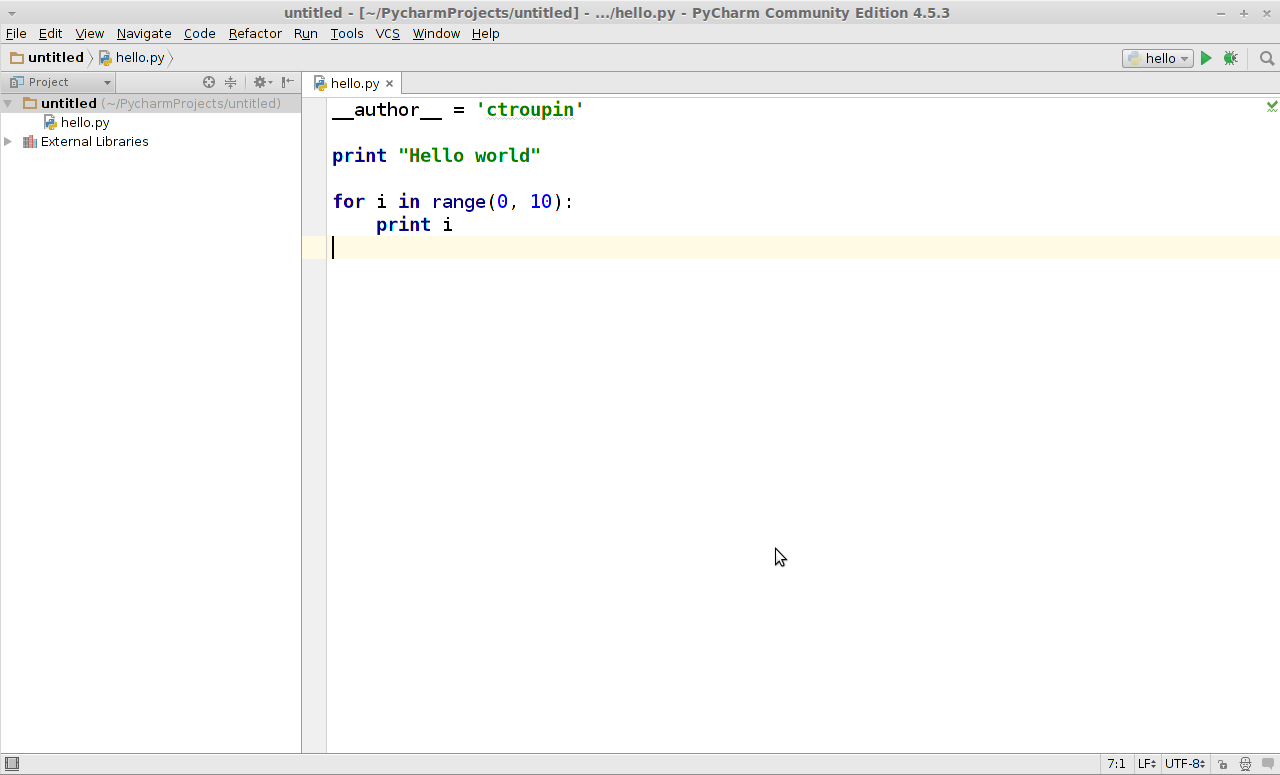
\includegraphics[width=.7\textwidth]{python_pycharm}
\vfill

\textbf{Examples:} Atom, Eclipse, PyCharm, Idle, \ldots\\
Complete list: \url{https://wiki.python.org/moin/PythonEditors}
\end{onlyenv}

\begin{onlyenv}<4>
\href{http://ipython.org/notebook.html}{\textit{ipython notebook}}\\
(interactive computational environment)

\vfill
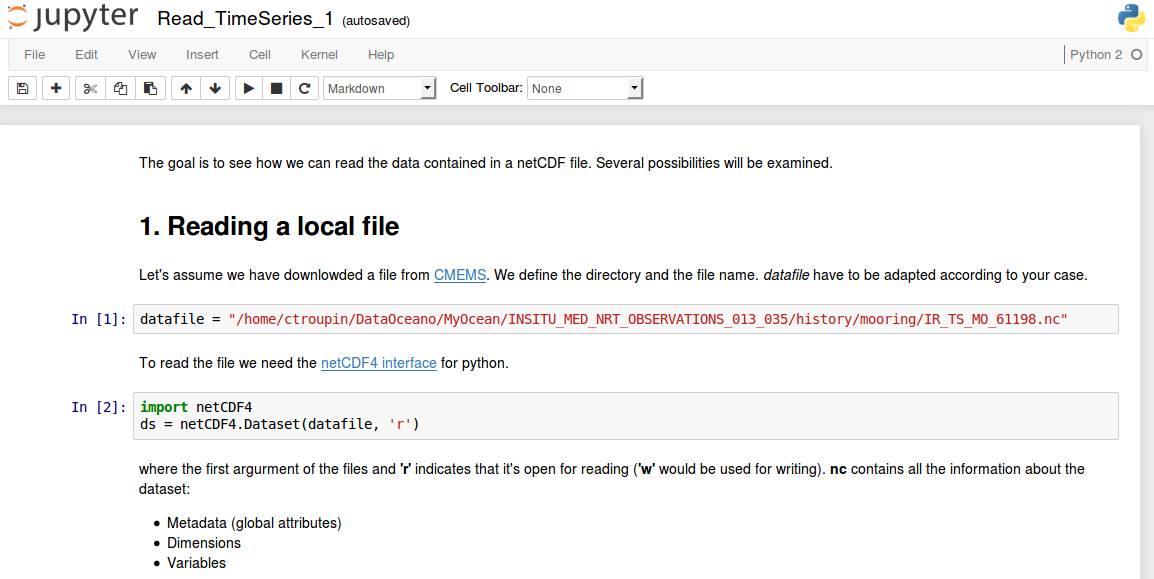
\includegraphics[width=.7\textwidth]{notebook_insitu0}
\vfill

Rich text + command executions + figures + \ldots

"\textit{Data story telling}"
\comment{(see Programming in Python 2)}
\end{onlyenv}

\end{frame}

%--------------------------------------------------------------------------------------------------------------
\begin{frame}[c]
\frametitle{What do we work with?}
\huge
\faLaptop

\vfill 

% Here we will say what we use personaly, type of workflow etc
\end{frame}

%--------------------------------------------------------------------------------------------------------------

\begin{frame}[c, fragile]
\frametitle{Exercise 1: changecase.py}

\exercise

Write a program that takes 2 arguments: the name and the surname, both written with a mix of upper and lowercase, and return the name with the first letter in uppercase and the surname with all the letters in uppercase.

\textbf{Examples:}

\textit{changecase allan rickman} \hspace{1cm} returns \hspace{1cm}  \textit{Allan RICKMAN} \\
\textit{changecase aLlAn ricKmaN} \hspace{1cm} returns \hspace{1cm}  \textit{Allan RICKMAN} 

\vspace{1cm}

\textbf{Tips:} use the function \href{https://docs.python.org/2/library/sys.html#sys.argv}{sys.argv} to be able to run the code as 
\begin{lstlisting}[language=bash]
$ changecase name surname
\end{lstlisting}


\end{frame}

